\documentclass[11pt]{amsart}
\usepackage[T1]{fontenc}
\usepackage{lmodern,microtype,amsmath,amssymb,amsthm,mathtools,enumitem}
\usepackage[margin=1in]{geometry}
\usepackage{graphicx}
\usepackage[hidelinks]{hyperref}
\newtheorem{mainthm}{Theorem}
\renewcommand{\themainthm}{\Alph{mainthm}}
\newtheorem{mainprop}[mainthm]{Proposition}
\newtheorem{theorem}{Theorem}[section]
\newtheorem{proposition}[theorem]{Proposition}
\newtheorem{lemma}[theorem]{Lemma}
\newtheorem{corollary}[theorem]{Corollary}
\theoremstyle{remark}
\newtheorem{remark}[theorem]{Remark}
\newcommand{\R}{\mathbb R}
\newcommand{\C}{\mathbb C}
\newcommand{\Z}{\mathbb Z}
\newcommand{\Rp}{\R_{+}}
\newcommand{\CH}{\C^{+}}
\DeclareMathOperator{\Log}{Log}
\DeclareMathOperator{\supp}{supp}
\hypersetup{pdftitle={Free multiplicative convolution and log-unimodality: three questions of Hasebe, Ueda and Wang},pdfauthor={Yitzchak Shmalo}}
\title[Log-unimodality and free multiplicative convolution]{Free multiplicative convolution and log-unimodality:\\ three questions of Hasebe, Ueda and Wang}
\author{Yitzchak Shmalo}
\address{Einstein Institute of Mathematics, The Hebrew University of Jerusalem, Jerusalem, Israel}
\date{11 October 2026}
\subjclass[2020]{46L54, 60E05}
\keywords{Free multiplicative convolution, log-unimodality, free multiplicative Brownian motion, strong unimodality}
\setlist{itemsep=3pt,topsep=5pt}
\setlength{\emergencystretch}{1em}
\raggedbottom
\begin{document}
\begin{abstract}
Hasebe, Ueda and Wang proved that free multiplicative convolution with the free positive multiplicative Brownian motion $\sigma_t$ preserves log-unimodality of multiplicatively symmetric laws, and asked three questions about how far this extends. We answer all three. The free multiplicative convolution of two multiplicatively symmetric log-unimodal laws need not be log-unimodal: for $L\ge6$, the logarithm of the free multiplicative square of the log-uniform law on $[e^{-L},e^{L}]$ has a density with a strict local minimum at $0$. Compact support of $\nu$ does not make $\sigma_t\boxtimes\nu$ log-unimodal for large $t$, since for $\nu=(\delta_{1/10}+\delta_{10})/2$ it fails for every $t>0$; when $\nu$ is in addition log-unimodal and supported in $[\alpha,\beta]$, the convolution is log-unimodal for all $t\ge(\pi/2)(\beta/\alpha+\alpha/\beta)$. Finally, $\sigma_t$ is not $\boxtimes$-strongly log-unimodal for any $t>0$, which extends the small-time result of Hasebe, Ueda and Wang to all times. The numerical inequalities behind the first and third answers and the root count behind the second are verified in Lean~4 with Mathlib.
\end{abstract}
\maketitle

\section{Introduction}

A Borel measure $\mu$ on $\R$ is \emph{unimodal} with mode $a$ if $\mu=c\,\delta_a+f(x)\,dx$ with $c\ge0$ and $f\ge0$ nondecreasing on $(-\infty,a)$ and nonincreasing on $(a,\infty)$. A probability measure $\mu$ on $\Rp=(0,\infty)$ is \emph{log-unimodal} if its image $\log_*\mu$ under $x\mapsto\log x$ is unimodal, and \emph{multiplicatively symmetric} if it is invariant under $x\mapsto x^{-1}$. For probability measures $\mu,\nu$ on $\Rp$ the free multiplicative convolution $\mu\boxtimes\nu$ is the law of $X^{1/2}YX^{1/2}$ for free positive operators $X,Y$ with laws $\mu,\nu$ \cite{Voi87,BV93}. The free positive multiplicative Brownian motion is the family $(\sigma_t)_{t>0}$ of $\boxtimes$-infinitely divisible laws with $\Sigma$-transform
\[
\Sigma_{\sigma_t}(z)=\exp\Bigl(\frac t2\,\frac{z+1}{z-1}\Bigr),
\]
introduced by Biane \cite{Bia98}. Zhong \cite{Zho15} described $\sigma_t\boxtimes\nu$ in detail; in particular it has a continuous density.

Hasebe, Ueda and Wang \cite{HUW} studied when $\sigma_t\boxtimes\nu$ is log-unimodal. They proved that it is whenever $\nu$ is multiplicatively symmetric and log-unimodal \cite[Theorem~4.2]{HUW}, and that it is for all $t\ge D$ when $\nu$ is supported in $[\alpha,\beta]$, $0<\alpha<\beta$, with $\beta^4-3\alpha^4<2\alpha^3\beta$ and $D$ an explicit constant \cite[Theorem~4.4]{HUW}. A probability measure $\mu$ on $\Rp$ is \emph{$\boxtimes$-strongly log-unimodal} if $\mu\boxtimes\nu$ is log-unimodal for every log-unimodal $\nu$; they proved that $\sigma_t$ is not $\boxtimes$-strongly log-unimodal for every $t$ in an interval $(0,t_0]$ \cite[Theorem~4.9]{HUW}. They asked the following three questions \cite[Problems~4.3, 4.7 and~4.11]{HUW}; numbering of \cite{HUW} follows its arXiv version.
\begin{enumerate}[label=\textup{(\arabic*)}]
\item ``If $\mu$ and $\nu$ are multiplicatively symmetric and log-unimodal on $\Rp$, is the free convolution $\mu\boxtimes\nu$ log-unimodal?''
\item ``Can we delete the assumption $\beta^4-3\alpha^4<2\alpha^3\beta$ in Theorem~4.4? More precisely, if $\nu$ is a probability measure supported on $[\alpha,\beta]$ such that $0<\alpha<\beta$, does there exist a number $D\ge0$ (depending on $\nu$) such that $\sigma_t\boxtimes\nu$ is log-unimodal for all $t\ge D$?''
\item ``Is it true that $\sigma_t$ is not $\boxtimes$-strongly log-unimodal for any $t>0$?''
\end{enumerate}
The answers are no, no, and yes. For $L>0$ let $\mu_L$ be the law of $e^U$ with $U$ uniform on $[-L,L]$,
\[
\mu_L(dx)=\frac{1}{2Lx}\,\mathbf 1_{[e^{-L},e^{L}]}(x)\,dx .
\]
It is multiplicatively symmetric and log-unimodal.

\begin{mainthm}\label{thm:A}
For every $L\ge6$ the measure $\mu_L\boxtimes\mu_L$ is not log-unimodal. More precisely, $\log_*(\mu_L\boxtimes\mu_L)$ has a real-analytic density on a neighbourhood of $0$, and this density has a strict local minimum at $0$.
\end{mainthm}

\begin{mainthm}\label{thm:B}
Let $\nu=\frac12(\delta_{1/10}+\delta_{10})$. Then $\sigma_t\boxtimes\nu$ is not log-unimodal for any $t>0$.
\end{mainthm}

\begin{mainthm}\label{thm:C}
For every $t>0$ there is a log-unimodal probability measure $\nu_t$ on $\Rp$, given explicitly in \eqref{eq:witness}, such that $\sigma_t\boxtimes\nu_t$ is not log-unimodal. Hence $\sigma_t$ is not $\boxtimes$-strongly log-unimodal for any $t>0$.
\end{mainthm}

The measure $\nu$ of Theorem~\ref{thm:B} does not satisfy the hypothesis of \cite[Theorem~4.4]{HUW}, since $10^4-3\cdot10^{-4}>2\cdot10^{-3}\cdot10$, and it is not log-unimodal. It is the failure of log-unimodality that matters: for log-unimodal $\nu$ the answer to the second question becomes positive, with a constant that depends only on the ratio $\beta/\alpha$.

\begin{mainprop}\label{prop:D}
Let $\nu$ be a log-unimodal probability measure supported in $[\alpha,\beta]$, $0<\alpha<\beta$. Then $\sigma_t\boxtimes\nu$ is log-unimodal for every
\[
t\ \ge\ \frac\pi2\Bigl(\frac\beta\alpha+\frac\alpha\beta\Bigr).
\]
\end{mainprop}

Proposition~\ref{prop:D} and \cite[Theorem~4.4]{HUW} do not contain each other: the former needs log-unimodality and no condition on $\beta/\alpha$, the latter a ratio $\beta/\alpha$ close to $1$ and no unimodality. Theorem~\ref{thm:B} also complements \cite[Theorem~4.5]{HUW}, where log-unimodality fails for all $t$ because atoms of $\nu$ escape to $0$ or $\infty$; here the support of $\nu$ is a fixed compact set.

The analogous large-time questions for the classical and free additive Brownian motions were settled by Hasebe and Ueda \cite{HU18}: started from a compactly supported law $\mu$, the free Brownian motion becomes unimodal after a time of the order of the square of the diameter of the support, while some initial laws are never unimodal; Hasebe and Sakuma \cite{HS17} proved large-time unimodality of free L\'evy processes whose L\'evy measure has bounded support and gave an unbounded counterexample. Theorem~\ref{thm:B} shows that the multiplicative analogue of the compactly supported statement fails without a unimodality assumption, and Proposition~\ref{prop:D} supplies the version with one. On the unit circle, Hasebe and Ueda \cite{HU21} proved that free multiplicative convolution with the free normal distributions preserves symmetric unimodality, that a symmetric law supported on an arc $\{e^{i\theta}:|\theta|\le\varphi\}$ with $\varphi<\pi/2$ becomes unimodal after a long time, and that the convolution of the symmetric Bernoulli law on $\{1,-1\}$ with a free normal distribution is unimodal at no time; this last example is the circle counterpart of Theorem~\ref{thm:B}. For recent work on the law $\sigma_t$ itself see \cite{Aue26}.

The proof of Theorem~\ref{thm:A} is complex-analytic. The $\eta$-transform of $\mu_L\boxtimes\mu_L$ has an explicit inverse on $(-\infty,0)$, and we show that this inverse inverts it on all of $\C\setminus[0,\infty)$. By multiplicative symmetry the $\eta$-transform maps the unit circle into itself, and its boundary value at the point $1$ can then be read off from the explicit inverse. Near $1$ the density of the logarithm is the imaginary part of an explicit analytic function, and the sign of its second derivative at $0$ reduces to the elementary inequality \eqref{eq:CL}. Theorems~\ref{thm:B} and~\ref{thm:C} and Proposition~\ref{prop:D} use Hasebe, Ueda and Wang's criterion \cite[Lemma~4.1]{HUW}, recalled in Lemma~\ref{lem:huw}: log-unimodality of $\sigma_t\boxtimes\nu$ is equivalent to a bound of two on the number of roots of a family of equations. For Theorem~\ref{thm:B} we exhibit four roots by the intermediate value theorem at every $t$. For Theorem~\ref{thm:C} the witness is an atom at $1$ together with a log-uniform law on a long interval $[e^{-\ell b},1]$, scaled with $t$ so that a single normalized equation has four roots for all $t$ at once.

The inequalities \eqref{eq:CL}, the root count of Theorem~\ref{thm:B} given the criterion, and the numerical inequalities and the choice of parameters in the proof of Theorem~\ref{thm:C} are verified in Lean~4 \cite{Lean} with Mathlib \cite{Mathlib}; Section~\ref{sec:lean} lists what is and is not formalized. Numerical computations, which are not used in any proof, show the shape of the densities involved (Figures~\ref{fig:A} and~\ref{fig:B}).

\section{Preliminaries}\label{sec:prelim}

For a probability measure $\lambda$ on $\Rp$ let
\[
\psi_\lambda(z)=\int_{\Rp}\frac{xz}{1-xz}\,\lambda(dx),\qquad \eta_\lambda(z)=\frac{\psi_\lambda(z)}{1+\psi_\lambda(z)},\qquad z\in\C\setminus[0,\infty).
\]
Both are analytic on $\C\setminus[0,\infty)$. For $z$ in the upper half-plane $\CH$ and $x>0$ we have $\operatorname{Im}\frac{xz}{1-xz}=\frac{x\operatorname{Im}z}{|1-xz|^2}>0$, so $\operatorname{Im}\psi_\lambda>0$ and $1+\psi_\lambda\ne0$ on $\CH$; since $\eta_\lambda=1-(1+\psi_\lambda)^{-1}$,
\begin{equation}\label{eq:etaH}
\operatorname{Im}\eta_\lambda(z)=\frac{\operatorname{Im}\psi_\lambda(z)}{|1+\psi_\lambda(z)|^2}>0\quad(z\in\CH),\qquad \eta_\lambda(z)\ne1\quad(z\in\C\setminus[0,\infty)).
\end{equation}
On $(-\infty,0)$ the function $\psi_\lambda$ takes values in $(-1,0)$, and $\eta_\lambda$ is an increasing bijection of $(-\infty,0)$ onto itself. Its inverse defines the $\Sigma$-transform $\Sigma_\lambda(z)=\eta_\lambda^{-1}(z)/z$, and $\Sigma_{\mu\boxtimes\nu}=\Sigma_\mu\Sigma_\nu$ on $(-\infty,0)$ \cite{Voi87,BV93}. The Cauchy transform $G_\lambda(\zeta)=\int(\zeta-x)^{-1}\lambda(dx)$ satisfies $1+\psi_\lambda(z)=z^{-1}G_\lambda(z^{-1})$, hence
\begin{equation}\label{eq:G}
G_\lambda(\zeta)=\frac{\zeta^{-1}}{1-\eta_\lambda(\zeta^{-1})}.
\end{equation}
Writing $\lambda^{-1}$ for the image of $\lambda$ under $x\mapsto x^{-1}$, a direct computation gives $\psi_{\lambda^{-1}}(z)=-1-\psi_\lambda(1/z)$, and therefore
\begin{equation}\label{eq:inv}
\eta_{\lambda^{-1}}(z)\,\eta_\lambda(1/z)=1 .
\end{equation}
Finally $(\mu\boxtimes\nu)^{-1}=\mu^{-1}\boxtimes\nu^{-1}$, because $(X^{1/2}YX^{1/2})^{-1}=X^{-1/2}Y^{-1}X^{-1/2}$ \cite[Section~4]{HUW}.

The next lemma is the form in which non-unimodality will be detected.

\begin{lemma}\label{lem:nomin}
Let $\lambda$ be a unimodal measure on $\R$ and $I$ an open interval on which $\lambda$ has a continuous density $g$. Then $g$ has no strict local minimum in $I$.
\end{lemma}

\begin{proof}
Let $\lambda=c\,\delta_m+f\,dx$ be as in the definition, so $f=g$ almost everywhere on $I$. Suppose $g(y)>g(y_0)$ for $0<|y-y_0|<\varepsilon$, with $(y_0-\varepsilon,y_0+\varepsilon)\subset I$. If $m\ge y_0$, then $f$ is nondecreasing on $(y_0-\varepsilon,y_0)$, so $g(y)\le g(y')$ for almost all $y<y'$ in that interval; letting $y'\uparrow y_0$ through such points and using continuity gives $g(y)\le g(y_0)$ for almost every $y\in(y_0-\varepsilon,y_0)$, a contradiction. If $m\le y_0$, the same argument on $(y_0,y_0+\varepsilon)$, where $f$ is nonincreasing, gives a contradiction.
\end{proof}

For $R\in(0,\pi)$ put
\[
\kappa_R(x)=\frac{1}{2(\cosh x-\cos R)},\qquad x\in\R .
\]
Since $\frac{r\xi}{1+r^2\xi^2-2r\xi\cos R}=\kappa_R(\log r+\log\xi)$, Hasebe, Ueda and Wang's criterion \cite[Lemma~4.1, (1)$\Leftrightarrow$(3)]{HUW} reads as follows in logarithmic coordinates. It rests on Zhong's description of $\sigma_t\boxtimes\nu$ \cite{Zho15}.

\begin{lemma}[Hasebe--Ueda--Wang]\label{lem:huw}
Let $t>0$ and let $\nu$ be a probability measure on $\Rp$. Then $\sigma_t\boxtimes\nu$ is log-unimodal if and only if for every $R\in(0,\pi)$ the equation
\begin{equation}\label{eq:huw}
\frac{\sin R}{R}\int_{\Rp}\kappa_R(x+\log\xi)\,\nu(d\xi)=\frac1t
\end{equation}
has at most two solutions $x\in\R$.
\end{lemma}

\section{Two log-uniform laws: proof of \texorpdfstring{Theorem~\ref{thm:A}}{Theorem A}}\label{sec:A}

Fix $L>0$, put $a=e^{-L}$, $\mu=\mu_L$ and $\rho=\mu\boxtimes\mu$. The support of $\rho$ is contained in $[a^2,a^{-2}]$, and $\rho$ is multiplicatively symmetric because $\mu$ is.

\subsection{The inverse of \texorpdfstring{$\eta_\rho$}{eta}}
Integrating,
\[
\psi_\mu(z)=\frac1{2L}\int_a^{1/a}\frac{z\,dx}{1-xz}=\frac1{2L}\Log\frac{1-az}{1-z/a},
\]
where $z\mapsto(1-az)/(1-z/a)$ maps $\C\setminus[a,1/a]$ into $\C\setminus(-\infty,0]$ and $\Log$ is the principal branch. Solving $\eta_\mu(z)=w$, that is $\psi_\mu(z)=w/(1-w)$, gives $\eta_\mu^{-1}=q_L$ on $(-\infty,0)$, where
\[
q_L(w)=\frac{1-E(w)}{a-E(w)/a},\qquad E(w)=\exp\Bigl(\frac{2Lw}{1-w}\Bigr).
\]
By the multiplicativity of $\Sigma$, the inverse of $\eta_\rho$ on $(-\infty,0)$ is
\begin{equation}\label{eq:QL}
Q_L(w)=\frac{q_L(w)^2}{w}.
\end{equation}
The function $q_L$ is meromorphic on $\C\setminus\{1\}$, with simple zeros where $E(w)=1$ (at $0$ and at the points $i\pi k/(L+i\pi k)$, $k\in\Z\setminus\{0\}$, all in the open unit disc) and simple poles where $E(w)=a^2$, that is at the points $w_k=1+iL/(\pi k)$, $k\in\Z\setminus\{0\}$; the point $1$ is an essential singularity. Hence $Q_L$ is meromorphic on $\C\setminus\{1\}$, analytic at $0$ with $Q_L(0)=0$, and its poles are the $w_k$. Let $P=\{1\}\cup\{w_k:k\ne0\}$, a closed set.

\begin{lemma}\label{lem:branch}
$Q_L(\eta_\rho(z))=z$ for every $z\in\C\setminus[0,\infty)$.
\end{lemma}

\begin{proof}
Let $\Omega_0=\C\setminus[0,\infty)$. By \eqref{eq:etaH}, $\eta_\rho$ never takes the value $1$ on $\Omega_0$. We claim that $Z=\eta_\rho^{-1}(P)$ is a discrete closed subset of $\Omega_0$. If $z_n\in Z$ converge to $z^*\in\Omega_0$, then $\eta_\rho(z^*)\in P$ since $P$ is closed, and $\eta_\rho(z^*)\ne1$, so $\eta_\rho(z^*)=w_k$ for some $k$. The point $w_k$ has a neighbourhood containing no other point of $P$, so for large $n$ we get $\eta_\rho(z_n)=w_k$, and as $\eta_\rho$ is not constant the $z_n$ are eventually equal to $z^*$. Thus $\Omega=\Omega_0\setminus Z$ is open and connected, and $Q_L\circ\eta_\rho$ is analytic on $\Omega$. It equals the identity on $(-\infty,0)\subset\Omega$ (the points of $(-\infty,0)$ are mapped into $(-\infty,0)$, which contains no pole), hence on $\Omega$. If $Z$ contained a point $z^*$, then $\eta_\rho(z^*)=w_k$ and $|Q_L(\eta_\rho(z))|\to\infty$ as $z\to z^*$, while $Q_L(\eta_\rho(z))=z$ stays bounded. So $Z=\emptyset$ and the identity holds on $\Omega_0$.
\end{proof}

\subsection{The unit circle}
By \eqref{eq:inv} with $\lambda=\rho=\rho^{-1}$, and since $\eta_\rho(\bar z)=\overline{\eta_\rho(z)}$, every $z$ on the unit circle other than $1$ satisfies $|\eta_\rho(z)|^2=\eta_\rho(z)\eta_\rho(1/z)=1$. As $\eta_\rho(-1)<0$, this gives $\eta_\rho(-1)=-1$.

On the circle the inverse $Q_L$ is explicit. For $w=e^{i\theta}$, $0<\theta<2\pi$, write $\theta=2s$. Then $\frac{w}{1-w}=-\frac12+\frac i2\cot s$, so $E(w)=a\,e^{i\varphi}$ with $\varphi=L\cot s$, and
\[
q_L(w)=-\frac1{B_a(e^{i\varphi})},\qquad B_a(v)=\frac{v-a}{1-av}.
\]
The Blaschke factor $B_a$ maps the unit circle onto itself; write $B_a(e^{i\varphi})=e^{i\beta_a(\varphi)}$ with $\beta_a$ continuous and $\beta_a(0)=0$. Then $\beta_a'(\varphi)=P_a(\varphi)$, where
\[
P_a(\varphi)=\frac{1-a^2}{D(\varphi)},\qquad D(\varphi)=1-2a\cos\varphi+a^2,
\]
and $\beta_a$ is odd, increasing, with $\beta_a(\pi)=\pi$. Consequently $Q_L(e^{i\theta})=e^{i\phi_L(\theta)}$ for $0<\theta<2\pi$, where
\[
\phi_L(\theta)=2\pi-\theta-2\beta_a\bigl(L\cot(\theta/2)\bigr),\qquad \phi_L'(\theta)=L\csc^2(\theta/2)\,P_a\bigl(L\cot(\theta/2)\bigr)-1 .
\]

\begin{lemma}\label{lem:phase}
If $L(1-a)/(1+a)>1$, then $\phi_L$ is an increasing bijection of $(0,2\pi)$ onto $\R$, and $\phi_L(\pi)=\pi$. Its zero $\theta_*=2s_*$ satisfies $s_*\in(s_0,\pi/2)$, where $s_0=\arctan(L/\pi)$, and $\varphi_*=L\cot s_*\in(0,\pi)$.
\end{lemma}

\begin{proof}
Since $P_a\ge(1-a)/(1+a)$ and $\csc^2\ge1$, we get $\phi_L'\ge L(1-a)/(1+a)-1>0$. As $\theta\downarrow0$, $L\cot(\theta/2)\to+\infty$ and $\beta_a\to+\infty$ (it increases by $2\pi$ over each period), so $\phi_L\to-\infty$; similarly $\phi_L\to+\infty$ as $\theta\uparrow2\pi$. Clearly $\phi_L(\pi)=\pi-2\beta_a(0)=\pi$. At $\theta=2s_0$ we have $L\cot s_0=\pi$ and $\phi_L(2s_0)=2\pi-2s_0-2\pi<0$, while $\phi_L(\pi)>0$; hence $s_*\in(s_0,\pi/2)$ and $\varphi_*\in(0,L\cot s_0)=(0,\pi)$.
\end{proof}

\begin{lemma}\label{lem:boundary}
Assume $L(1-a)/(1+a)>1$ and put $w_*=e^{i\theta_*}$. Then $\eta_\rho(e^{i\gamma})=e^{i\phi_L^{-1}(\gamma)}$ for $0<\gamma<2\pi$; in particular $\eta_\rho(e^{i\gamma})\to w_*$ as $\gamma\downarrow0$. Moreover $Q_L$ is analytic at $w_*$ with $Q_L(w_*)=1$ and $Q_L'(w_*)=A/w_*$, where
\[
A=\phi_L'(\theta_*)=L\csc^2 s_*\,P_a(\varphi_*)-1>0 .
\]
\end{lemma}

\begin{proof}
Since $\eta_\rho$ is continuous on the circle minus $1$, has modulus one there and never equals $1$, we can write $\eta_\rho(e^{i\gamma})=e^{i\vartheta(\gamma)}$ with $\vartheta:(0,2\pi)\to(0,2\pi)$ continuous. The poles $w_k$ have modulus larger than one, so Lemma~\ref{lem:branch} gives $e^{i\phi_L(\vartheta(\gamma))}=e^{i\gamma}$. The continuous function $\phi_L(\vartheta(\gamma))-\gamma$ takes values in $2\pi\Z$ and vanishes at $\gamma=\pi$, because $\vartheta(\pi)=\pi$; so $\vartheta=\phi_L^{-1}$ on $(0,2\pi)$, and $\vartheta(\gamma)\to\phi_L^{-1}(0)=\theta_*$ as $\gamma\downarrow0$. The point $w_*\ne1$ lies on the circle, away from the poles, and differentiating $Q_L(e^{i\theta})=e^{i\phi_L(\theta)}$ at $\theta_*$ gives $Q_L'(w_*)=\phi_L'(\theta_*)/w_*$.
\end{proof}

\subsection{The density near \texorpdfstring{$1$}{1}}
Assume $L(1-a)/(1+a)>1$. By Lemma~\ref{lem:boundary} and the inverse function theorem there are a neighbourhood $U$ of $w_*$ and a disc $\Delta=\{|z-1|<\delta\}$ such that $Q_L$ maps $U$ biholomorphically onto $\Delta$; let $H:\Delta\to U$ be the inverse, $H(1)=w_*$. For small $\gamma>0$ both $\eta_\rho(e^{i\gamma})$ and $H(e^{i\gamma})$ lie in $U$ and are mapped by $Q_L$ to $e^{i\gamma}$, so they coincide. The arc $\{e^{i\gamma}\}$ accumulates inside the connected open set $\Delta\cap\CH$, where $\eta_\rho$ and $H$ are analytic, hence
\begin{equation}\label{eq:etaH2}
\eta_\rho=H\quad\text{on }\Delta\cap\CH .
\end{equation}
Thus $\eta_\rho$ extends continuously from $\CH$ to the segment $(1-\delta,1+\delta)$ with values $H(x)$, and by reflection from the lower half-plane with values $\overline{H(x)}$. By \eqref{eq:G}, $G_\rho$ extends continuously from $\CH$ to the real points $x$ with $x^{-1}\in(1-\delta,1+\delta)$, where $G_\rho(x+i0)=x^{-1}\bigl(1-\overline{H(x^{-1})}\bigr)^{-1}$; note $H\ne1$ near $1$ because $w_*\ne1$. By Stieltjes inversion, $\rho$ has there the continuous density $-\pi^{-1}\operatorname{Im}G_\rho(x+i0)$, and $\log_*\rho$ has, for $|y|<\log(1+\delta)$, the density
\begin{equation}\label{eq:g}
g(y)=\frac1\pi\operatorname{Im}\frac1{1-H(e^{-y})}.
\end{equation}
It is real-analytic, and even because $\rho$ is multiplicatively symmetric.

\begin{proposition}\label{prop:g}
In this situation,
\[
g(0)=\frac{\cot s_*}{2\pi},\qquad g'(0)=0,\qquad g''(0)=-\frac{\csc^2s_*}{4\pi A^3}\,\bigl(B+A\cot s_*\bigr),
\]
where $B=\phi_L''(\theta_*)$. Explicitly,
\begin{equation}\label{eq:B}
B+A\cot s_*=-\cot s_*+\frac{L^2a(1-a^2)\sin\varphi_*}{D(\varphi_*)^2\sin^4s_*}.
\end{equation}
\end{proposition}

\begin{proof}
Let $\Phi$ be the analytic continuation of $\phi_L$ to a complex neighbourhood of $\theta_*$; then $Q_L(e^{i\tau})=e^{i\Phi(\tau)}$ there. Put $w(y)=H(e^{-y})$ and $w(y)=e^{i\tau(y)}$ with $\tau(0)=\theta_*$. From $Q_L(w(y))=e^{-y}$ and $\Phi(\theta_*)=0$ we get $\Phi(\tau(y))=iy$, so $\tau'(0)=i/A$ and $\tau''(0)=-\Phi''(\theta_*)\tau'(0)^2/A=B/A^3$. Hence
\[
w'(0)=i\tau'(0)w_*=-\frac{w_*}A,\qquad w''(0)=w_*\bigl(i\tau''(0)-\tau'(0)^2\bigr)=\frac{w_*(A+iB)}{A^3}.
\]
With $F(w)=(1-w)^{-1}$ and $1-w_*=-2i\sin s_*\,e^{is_*}$,
\[
F(w_*)=\tfrac12+\tfrac i2\cot s_*,\qquad F'(w_*)=-\frac{e^{-2is_*}}{4\sin^2s_*},\qquad F''(w_*)=\frac{2}{8i\sin^3s_*\,e^{3is_*}} .
\]
The first identity gives $g(0)$. Next $\pi g'(0)=\operatorname{Im}F'(w_*)w'(0)=\operatorname{Im}\frac{1}{4A\sin^2s_*}=0$. Finally
\[
\pi g''(0)=\operatorname{Im}\bigl(F''(w_*)w'(0)^2+F'(w_*)w''(0)\bigr)=\operatorname{Im}\Bigl(\frac{-ie^{is_*}}{4A^2\sin^3s_*}-\frac{A+iB}{4A^3\sin^2s_*}\Bigr)=-\frac{A\cot s_*+B}{4A^3\sin^2s_*}.
\]
For \eqref{eq:B}, differentiate $\phi_L'(\theta)=L\csc^2(\theta/2)P_a(L\cot(\theta/2))-1$, using $\frac{d}{d\theta}\csc^2\frac\theta2=-\csc^2\frac\theta2\cot\frac\theta2$, $\frac{d}{d\theta}L\cot\frac\theta2=-\frac L2\csc^2\frac\theta2$ and $P_a'(\varphi)=-2a(1-a^2)\sin\varphi/D(\varphi)^2$:
\[
B=-L\csc^2s_*\cot s_*\,P_a(\varphi_*)+\frac{L^2a(1-a^2)\sin\varphi_*}{D(\varphi_*)^2\sin^4s_*},
\]
and $A\cot s_*=L\csc^2s_*\cot s_*\,P_a(\varphi_*)-\cot s_*$.
\end{proof}

\begin{lemma}\label{lem:CL}
For every real $L\ge6$, with $a=e^{-L}$,
\begin{equation}\label{eq:CL}
a(1-a^2)(L^2+\pi^2)^2<L(1-a)^4\qquad\text{and}\qquad L\,\frac{1-a}{1+a}>1 .
\end{equation}
\end{lemma}

\begin{proof}
The second inequality is clear. For the first write $L=s+6$ with $s\ge0$ and $T(s)=1+s+\frac{s^2}2+\frac{s^3}6+\frac{s^4}{24}\le e^s$. Since $e>\frac{1359}{500}$ we have $e^6>400$, so $a<\frac1{400}$ and $(1-a)^4\ge(\frac{399}{400})^4$; also $\pi^2<10$. Hence
\[
a(1-a^2)(L^2+\pi^2)^2<\frac{(L^2+10)^2}{e^6e^s}<\frac{(L^2+10)^2}{400\,T(s)},
\]
and it suffices to show $(L^2+10)^2\le c\,L\,T(s)$ with $c=399^4/400^3$. The difference $c(s+6)T(s)-((s+6)^2+10)^2$ is a polynomial in $s$ with coefficients
\[
6c-2116,\quad 7c-1104,\quad 4c-236,\quad \tfrac32c-24,\quad \tfrac5{12}c-1,\quad \tfrac1{24}c
\]
of $1,s,\dots,s^5$, all positive because $c=400(1-\frac1{400})^4\ge396$ by Bernoulli's inequality.
\end{proof}

\begin{proof}[Proof of Theorem~\ref{thm:A}]
Let $L\ge6$. By Lemma~\ref{lem:CL}, Lemmas~\ref{lem:phase} and~\ref{lem:boundary} and Proposition~\ref{prop:g} apply. In \eqref{eq:B} use $\sin\varphi_*<\varphi_*=L\cot s_*$, $D(\varphi_*)\ge(1-a)^2$, and $\sin s_*>\sin s_0=L/\sqrt{L^2+\pi^2}$, which holds because $s_0<s_*<\pi/2$. Since $\cot s_*>0$,
\[
B+A\cot s_*<\cot s_*\bigl(C_L-1\bigr),\qquad C_L=\frac{a(1-a^2)(L^2+\pi^2)^2}{L(1-a)^4},
\]
and $C_L<1$ by \eqref{eq:CL}. Hence $g''(0)>0$. The density $g$ of $\log_*\rho$ is continuous near $0$, even, and has $g'(0)=0<g''(0)$, so it has a strict local minimum at $0$. By Lemma~\ref{lem:nomin}, $\log_*\rho$ is not unimodal.
\end{proof}

\begin{remark}[Numerics]\label{rem:numA}
For $L=6$ one finds $s_*=1.268996$, $w_*=-0.823297+0.567611\,i$, $A=5.571866$, $B=-1.943520$, $B+A\cot s_*=-0.208942$ and $C_6=0.877891$, so that $g(0)=0.049547$ and $g''(0)=1.0544\times10^{-4}$. The point $w_*$ given by Lemma~\ref{lem:boundary} agrees to $1.6\times10^{-16}$ with the boundary value of $\eta_\rho$ at $1$ obtained by solving the subordination equations of Belinschi and Bercovici \cite{BB07} at $z=1+i\varepsilon$ and letting $\varepsilon\downarrow0$. The whole density $g$ is shown in Figure~\ref{fig:A}: for $L=6$ it is supported in $[-10.307,10.307]$, has total mass $1$ to six decimals, and its maximum $0.051180$ is attained at $\pm6.674$, so $g(0)$ is $0.968$ times the maximum. A random-matrix check agrees: for $N=1000$, the logarithms of the eigenvalues of $X^{1/2}UYU^*X^{1/2}$, with $X,Y$ diagonal with entries $e^{u_i}$, $u_i$ the midpoints of $N$ equal cells of $[-6,6]$, and $U$ Haar-distributed unitary, so that $X$ and $UYU^*$ are asymptotically free \cite{Voi91}, have, over $16$ samples, window averages within $10^{-4}$ of those of $g$, and the same dip.

The numerics also locate the transition. The sign of $g''(0)$ changes at $L_c=3.354645$; for $L=2$ and $L=3$ the computed density has a single peak at $0$, while for $L=3.5,4,5,6,8,10,12$ its maximum sits at $\pm1.185,\pm2.661,\pm4.764,\pm6.674,\pm10.423,\pm14.193,\pm17.997$. This suggests that $\mu_L\boxtimes\mu_L$ is log-unimodal exactly when $L\le L_c$; we prove only the case $L\ge6$ of the failure.
\end{remark}

\begin{figure}[t]
\centering
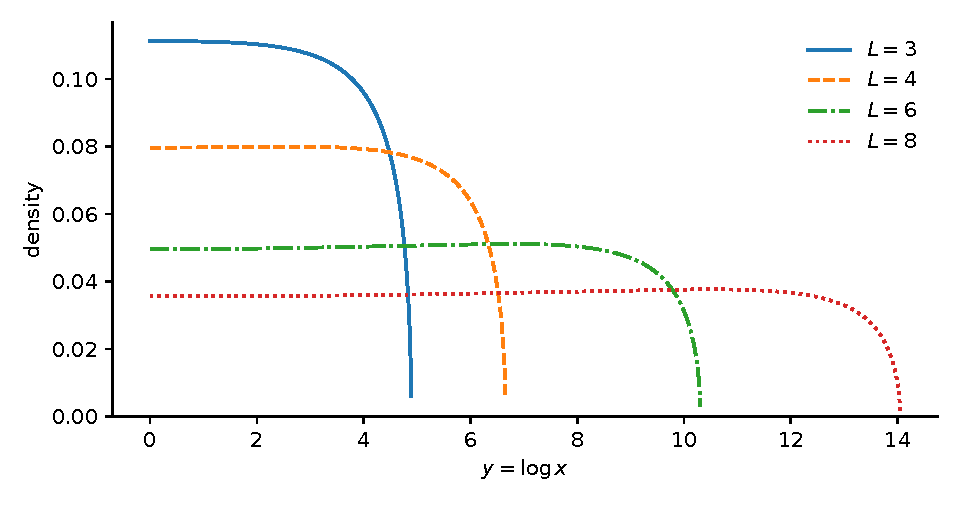
\includegraphics[width=0.82\textwidth]{fig_loguniform.pdf}
\caption{The density $g$ of $\log_*(\mu_L\boxtimes\mu_L)$ for $L=3,4,6,8$. For $L=3$ the density is unimodal; for $L=4,6,8$ it has a local minimum at $0$ (computed numerically; Theorem~\ref{thm:A} proves the minimum for $L\ge6$).}
\label{fig:A}
\end{figure}

\section{Two atoms: proof of \texorpdfstring{Theorem~\ref{thm:B} and Proposition~\ref{prop:D}}{Theorem B and Proposition D}}\label{sec:B}

\subsection{\texorpdfstring{Theorem~\ref{thm:B}}{Theorem B}}
Let $\nu=\frac12(\delta_{1/10}+\delta_{10})$ and, for $R\in(0,\pi)$ and $r>0$,
\[
k_R(x)=\frac{x}{1+x^2-2x\cos R},\qquad F_R(r)=\frac12\bigl(k_R(r/10)+k_R(10r)\bigr),
\]
so that \eqref{eq:huw} with $x=\log r$ reads $\frac{\sin R}{R}F_R(r)=\frac1t$.

\begin{lemma}\label{lem:window}
Let $R\in(0,\pi)$ and $\frac18\le\lambda\le\frac1{4-4\cos R}$. Then $F_R(r)=\lambda$ has a solution in each of the intervals $(\frac1{1000},\frac1{10})$, $(\frac1{10},1)$, $(1,10)$ and $(10,1000)$.
\end{lemma}

\begin{proof}
Since $k_R(1/x)=k_R(x)$, we have $F_R(1/r)=F_R(r)$. Using $k_R(x)\le x/(1-x)^2$ for $0<x<1$, $F_R(\frac1{1000})=F_R(1000)\le\frac12\bigl(\frac{10^{-4}}{(1-10^{-4})^2}+\frac{10^{-2}}{(1-10^{-2})^2}\bigr)<\frac18$. Next $F_R(\frac1{10})=F_R(10)>\frac12k_R(1)=\frac1{4-4\cos R}$, and $F_R(1)=k_R(10)=\frac{1}{10.1-2\cos R}\le\frac{10}{81}<\frac18$. The function $F_R$ is continuous, so the intermediate value theorem gives the four solutions.
\end{proof}

\begin{proof}[Proof of Theorem~\ref{thm:B}]
Fix $t>0$. If $t\le8$, take $R=\sqrt t/2\in(0,\sqrt2\,]$. The level $\lambda=\frac{R}{t\sin R}=\frac{1}{4R\sin R}$ satisfies $\lambda\ge\frac18$ because $R\sin R\le\sqrt2$, and $\lambda\le\frac1{4-4\cos R}$ because $1-\cos R\le R\sin R$, which is $\tan\frac R2\le R$ and holds for $R\le\sqrt2$. If $t>8$, take $R\in(0,\pi)$ with $\frac{\sin R}{R}=\frac8t$, which exists because $\frac{\sin R}R$ decreases from $1$ to $0$; then $\lambda=\frac18\le\frac1{4-4\cos R}$. In both cases Lemma~\ref{lem:window} gives four solutions of $\frac{\sin R}RF_R(r)=\frac1t$, so $\sigma_t\boxtimes\nu$ is not log-unimodal by Lemma~\ref{lem:huw}.
\end{proof}

\begin{remark}[The shape of the density]\label{rem:numB}
Zhong's description \cite{Zho15} shows how the failure looks. The set $V_{t,\nu}=\{r>0:\int\frac{r\xi}{(1-r\xi)^2}\nu(d\xi)>\frac1t\}$ is mapped by a homeomorphism onto the set of reciprocals of the points where the density of $\sigma_t\boxtimes\nu$ is positive, and the support is the closure of that set. Here the integral equals $\frac12\bigl(\frac14\operatorname{csch}^2\frac{u-\log10}{2}+\frac14\operatorname{csch}^2\frac{u+\log10}{2}\bigr)$ with $u=\log r$; it is convex in $u$ on $(-\log10,\log10)$, increasing in $r$ on $(0,\frac1{10})$, decreasing on $(10,\infty)$, and takes the value $\frac{10}{81}$ at $r=1$. So for $t<\frac{81}{10}$ the support of $\sigma_t\boxtimes\nu$ consists of two intervals, and the logarithmic density vanishes on an interval $(-Y_t,Y_t)$; numerically $Y_t=1.999,1.421,0.749,0.333,0.106,0.001$ for $t=0.05,0.5,2,4,6,8$. For $t\ge\frac{81}{10}$ the support is an interval; at $t=\frac{81}{10}$ the density of the logarithm vanishes only at $0$, and for larger $t$ the failure is a dip: the density of the logarithm at $0$ is $0.460,0.721,0.868,0.921,0.959$ times its maximum for $t=10,5\pi,30,50,100$ (Figure~\ref{fig:B}). For a symmetric unimodal density the value at $0$ is the maximum, so these ratios show the failure directly, and they tend to $1$ slowly as $t$ grows.
\end{remark}

\begin{figure}[t]
\centering
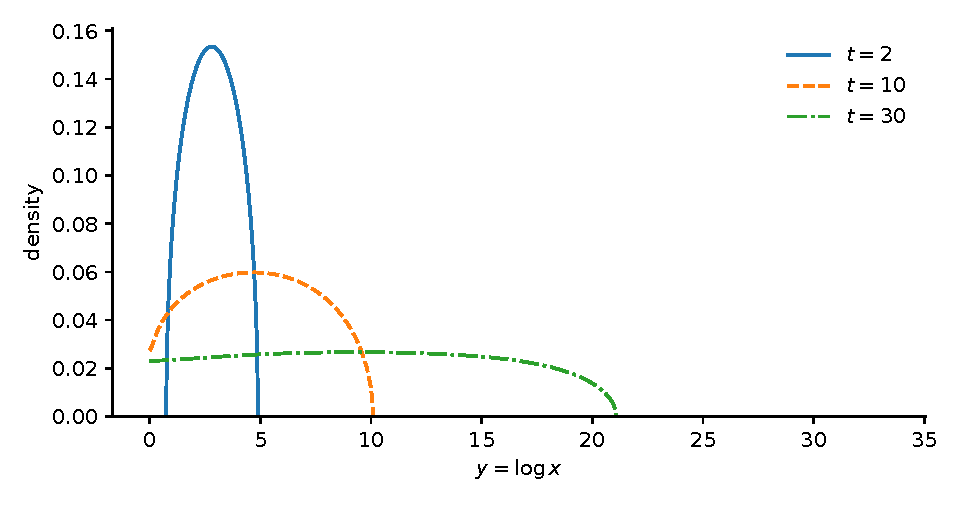
\includegraphics[width=0.82\textwidth]{fig_twoatoms.pdf}
\caption{The density of $\log_*(\sigma_t\boxtimes\nu)$ for $\nu=\frac12(\delta_{1/10}+\delta_{10})$ and $t=2,10,30$, computed numerically from Zhong's formula. For $t=2$ the support has a gap around $0$; for $t=10$ and $t=30$ the density is positive at $0$ but below its maximum.}
\label{fig:B}
\end{figure}

\subsection{\texorpdfstring{Proposition~\ref{prop:D}}{Proposition D}}

\begin{proof}[Proof of Proposition~\ref{prop:D}]
Let $m=\log_*\nu$, supported in $[a_1,a_2]=[\log\alpha,\log\beta]$, and $w=a_2-a_1$, so that $\frac\pi2(\frac\beta\alpha+\frac\alpha\beta)=\pi\cosh w$. Fix $t\ge\pi\cosh w$ and $R\in(0,\pi)$, and let
\[
h(x)=\int\kappa_R(x+s)\,m(ds),\qquad x\in\R .
\]
By Lemma~\ref{lem:huw} we must show that $\frac{\sin R}R\,h(x)=\frac1t$ has at most two solutions. The function $h$ extends analytically to a strip around $\R$, because $m$ has compact support, and $h(x)\to0$ as $|x|\to\infty$; so $h$ is not constant on any interval.

Suppose $R\ge\pi/2$, and write $c=-\cos R\ge0$. Then $(\log(\cosh x+c))''=\frac{1+c\cosh x}{(\cosh x+c)^2}>0$, so $\kappa_R$ is log-concave, and since $\int\kappa_R=\frac{\pi-R}{\sin R}$ the function $\frac{\sin R}{\pi-R}\kappa_R$ is a log-concave probability density. The image of $m$ under $s\mapsto-s$ is unimodal, and by Ibragimov's theorem \cite{Ibr56} its convolution with $\frac{\sin R}{\pi-R}\kappa_R$ is unimodal; this convolution is $\frac{\sin R}{\pi-R}\,h$. A unimodal continuous function that is not constant on any interval is strictly increasing to the left of its mode and strictly decreasing to the right, so each level is attained at most twice.

Suppose $R<\pi/2$. For $x\le-a_2$ every $x+s$ with $s\in[a_1,a_2]$ is $\le0$, where $\kappa_R$ is strictly increasing; so $h$ is strictly increasing on $(-\infty,-a_2]$, and likewise strictly decreasing on $[-a_1,\infty)$. For $x\in[-a_2,-a_1]$ we have $|x+s|\le w$, hence $h(x)\ge\kappa_R(w)$ and
\[
\frac{\sin R}R\,h(x)\ \ge\ \frac{\sin R}{2R(\cosh w-\cos R)}=\frac1{f(R)},\qquad f(R)=\frac{2R(\cosh w-1)}{\sin R}+2R\tan\frac R2 .
\]
Both terms of $f$ increase on $(0,\pi/2)$, so $f(R)<f(\pi/2)=\pi\cosh w\le t$. Thus there is no solution in $[-a_2,-a_1]$ and at most one on each side.
\end{proof}

The case $R<\pi/2$ uses only the support of $\nu$. For the measure of Theorem~\ref{thm:B} it excludes a middle root at every $R<\pi/2$ once $t\ge\pi\cosh(\log100)\approx157$, and indeed the angle used in the proof of Theorem~\ref{thm:B} exceeds $\pi/2$ for every $t>4\pi$. At such angles the root count is governed by the case $R\ge\pi/2$, which is where log-unimodality of $\nu$ enters.

\section{All times: proof of \texorpdfstring{Theorem~\ref{thm:C}}{Theorem C}}\label{sec:C}

For $0<b<\pi$ and $v\in\R$ let
\[
K_b(v)=\frac{b\sin b}{2\pi(\cosh(bv)-\cos b)}=\frac{b\sin b}{\pi}\,\kappa_b(bv),\qquad K_0(v)=\frac1{\pi(1+v^2)} .
\]

\begin{lemma}\label{lem:kernel}
For fixed $v$, $b\mapsto K_b(v)$ is nonincreasing on $(0,\pi)$, and $K_b(v)\le K_0(v)$. Moreover
\begin{equation}\label{eq:primitive}
\int_u^vK_b=\frac{\Phi_b(v)-\Phi_b(u)}\pi,\qquad \Phi_b(v)=\arctan\Bigl(\cot\frac b2\,\tanh\frac{bv}2\Bigr).
\end{equation}
\end{lemma}

\begin{proof}
Since $1-\cos b=\sin b\tan\frac b2$,
\[
\frac{1}{2\pi K_b(v)}=\frac{\cosh(bv)-\cos b}{b\sin b}=v^2\,\frac{\cosh(bv)-1}{(bv)^2}\cdot\frac b{\sin b}+\frac{\tan(b/2)}b
\]
(the first term read as $0$ when $v=0$). Each factor is nonnegative and nondecreasing in $b\in(0,\pi)$: $(\cosh x-1)/x^2$ is even and nondecreasing in $x\ge0$, because $x\sinh x-2(\cosh x-1)$ vanishes at $0$ with derivative $x\cosh x-\sinh x\ge0$; $b/\sin b$ has derivative $(\sin b-b\cos b)/\sin^2b>0$; and $\tan x/x$ increases on $(0,\pi/2)$. So $K_b(v)$ is nonincreasing in $b$, and letting $b\downarrow0$ gives $K_b\le K_0$. For \eqref{eq:primitive}, multiply numerator and denominator of $\Phi_b'(v)$ by $\sin^2\frac b2\cosh^2\frac{bv}2$ and use $\sin^2\frac b2+\sinh^2\frac{bv}2=\frac12(\cosh(bv)-\cos b)$; this gives $\Phi_b'=\pi K_b$.
\end{proof}

For $b\in(0,\pi)$, $\ell>0$ and $p\in(0,1)$ let $\nu_{b,\ell,p}$ be the probability measure on $\Rp$ with
\begin{equation}\label{eq:witness0}
\log_*\nu_{b,\ell,p}=p\,\delta_0+\frac{1-p}{\ell b}\,\mathbf 1_{[-\ell b,0]}(s)\,ds .
\end{equation}
It is log-unimodal with mode $1$. Substituting $s=b(v-y)$, the left side of \eqref{eq:huw} at $R=b$ and $x=by$ equals $\frac\pi{b^2}S(y)$, where
\[
S(y)=p\,K_b(y)+\frac{1-p}\ell\int_{y-\ell}^yK_b(v)\,dv .
\]

\begin{lemma}\label{lem:crossing}
Let $0<b\le\frac1{10}$, $\ell\ge100$, $p=\frac8{5\ell}$, and $W=\ell S$. Then
\[
W(0)>\tfrac{19}{20},\qquad W(3)<\tfrac{19}{20},\qquad W(\ell/2)>\tfrac{19}{20}.
\]
\end{lemma}

\begin{proof}
Here $W(y)=\frac85K_b(y)+(1-\frac8{5\ell})\int_{y-\ell}^yK_b$ and $1-\frac8{5\ell}\ge\frac{123}{125}$. We use $\cot\frac1{20}>\frac{799}{40}$, from $\cos x>1-\frac{x^2}2$ and $\sin x<x$; $\tanh5>\frac9{10}$ and $\tanh\frac52>\frac{29}{30}$, equivalent to $e^{10}>19$ and $e^5>59$; and $\arctan x>\frac\pi2-\frac1x$ for $x>0$. Write $X=\cot\frac1{20}$.

At $y=0$, Lemma~\ref{lem:kernel} with $K_b\ge K_{1/10}$ and $\ell\ge100$ gives, using $K_{1/10}(0)=\frac{X}{20\pi}$ and \eqref{eq:primitive},
\[
W(0)\ge\frac{2X}{25\pi}+\frac{123}{125\pi}\arctan\bigl(X\tanh5\bigr).
\]
Since $X\tanh5>\frac{7191}{400}$, the right side exceeds $\frac{19}{20}$ as soon as $\frac{799}{500}-\frac{123}{125}\cdot\frac{400}{7191}>\frac{229}{500}\pi$, which holds because $\pi<\frac{63}{20}$.

At $y=3$, Lemma~\ref{lem:kernel} with $K_b\le K_0$ gives
\[
W(3)\le\frac85K_0(3)+\int_{-\infty}^3K_0=1-\frac{\arctan(1/3)}\pi+\frac4{25\pi},
\]
which is less than $\frac{19}{20}$ because $\arctan\frac13>\frac13-\frac1{81}=\frac{26}{81}>\frac{11}{70}+\frac4{25}>\frac\pi{20}+\frac4{25}$, the last step by $\pi<\frac{22}7$.

At $y=\ell/2$, drop the first term; since $[-50,50]\subset[-\ell/2,\ell/2]$,
\[
W(\ell/2)\ge\frac{123}{125}\int_{-50}^{50}K_{1/10}=\frac{246}{125\pi}\arctan\Bigl(X\tanh\frac52\Bigr).
\]
Since $X\tanh\frac52>\frac{23171}{1200}$, this exceeds $\frac{19}{20}$ as soon as $\frac{17}{500}\pi>\frac{246}{125}\cdot\frac{1200}{23171}$, which holds because $\pi>3$.
\end{proof}

\begin{proof}[Proof of Theorem~\ref{thm:C}]
Fix $t>0$ and set
\[
\ell=\max\{100,\,95\pi t\},\qquad b=\sqrt{\frac{19\pi t}{20\,\ell}},\qquad p=\frac8{5\ell},
\]
and let
\begin{equation}\label{eq:witness}
\nu_t=\nu_{b,\ell,p}.
\end{equation}
Since $\ell\ge95\pi t$ we have $b^2\le\frac1{100}$, so Lemma~\ref{lem:crossing} applies; also $p\le\frac2{125}$. As $|y|\to\infty$, $W(y)\to0$. Hence $W=\frac{19}{20}$ has a solution in each of $(-\infty,0)$, $(0,3)$, $(3,\ell/2)$ and $(\ell/2,\infty)$. At such a solution $S(y)=\frac{19}{20\ell}=\frac{b^2}{\pi t}$, so the left side of \eqref{eq:huw} at $R=b$ and $x=by$ equals $\frac1t$. Equation \eqref{eq:huw} thus has four solutions, and $\sigma_t\boxtimes\nu_t$ is not log-unimodal by Lemma~\ref{lem:huw}.
\end{proof}

The support of $\nu_t$ is $[e^{-\ell b},1]$, and $\ell b=\sqrt{19\pi t\ell/20}\ge\frac{19}{2}\pi t$. So Proposition~\ref{prop:D} would require $t\ge\pi\cosh(\ell b)$, far beyond $t$; the two results are consistent, and the witnesses must spread out on the logarithmic scale as $t$ grows.

\section{Lean verification and computations}\label{sec:lean}

The file \texttt{LogUnimodality.lean} in the repository listed below checks the following parts of the proofs in Lean~4 \cite{Lean} with Mathlib \cite{Mathlib} (toolchain v4.33.1). Every statement is about explicit real numbers or real functions, and the only axioms used are the standard ones (\texttt{propext}, \texttt{Classical.choice}, \texttt{Quot.sound}).
\begingroup\sloppy
\begin{itemize}
\item \texttt{thmA\_core}: both inequalities \eqref{eq:CL} for every real $L\ge6$.
\item \texttt{k\_exp}, \texttt{four\_roots\_of\_window}, \texttt{level\_small}, \texttt{level\_large} and \texttt{thmB\_four\_roots}: the identity $k_R(e^u)=\kappa_R(u)$, Lemma~\ref{lem:window} (with the four roots ordered rather than located), the two choices of $R$ in the proof of Theorem~\ref{thm:B}, and, for every $t>0$, the existence of $R\in(0,\pi)$ and of four positive numbers $r_1<r_2<r_3<r_4$ with $\frac{\sin R}{R}F_R(r_i)=\frac1t$. Together with Lemma~\ref{lem:huw} this is Theorem~\ref{thm:B}. \texttt{thm44\_hypothesis\_fails} checks that $\nu$ violates the hypothesis of \cite[Theorem~4.4]{HUW}.
\item \texttt{K\_B\_zero}, \texttt{arctan\_third}, \texttt{crossing\_zero}, \texttt{crossing\_three}, \texttt{crossing\_mid} and \texttt{parameters}: the value $K_{1/10}(0)=\frac{X}{20\pi}$, the bound $\arctan\frac13>\frac\pi{20}+\frac4{25}$, the three numerical inequalities in the proof of Lemma~\ref{lem:crossing}, and the properties of $\ell,b,p$ used in the proof of Theorem~\ref{thm:C}.
\end{itemize}
\endgroup
Not formalized are the free-probability input (the transforms, Lemma~\ref{lem:huw}, the branch and boundary arguments of Section~\ref{sec:A}), Lemma~\ref{lem:nomin}, Lemma~\ref{lem:phase}, Proposition~\ref{prop:g} and the estimate of $B+A\cot s_*$ through $C_L$ in the proof of Theorem~\ref{thm:A}, Lemma~\ref{lem:kernel} and its use in the proof of Lemma~\ref{lem:crossing}, and Proposition~\ref{prop:D}. An independent check of the rational inequalities of Lemma~\ref{lem:crossing} in exact arithmetic is included. The scripts behind Remarks~\ref{rem:numA} and~\ref{rem:numB} and the figures compute the densities from Zhong's formula and from the subordination equations; their outputs are in the repository.

\section*{Acknowledgements and funding}
The research presented in this paper was supported by the European Research
Council (ERC) under the European Union's Horizon Europe research and
innovation programme (grant agreement No.~101041711), by the Simons
Foundation as part of the Collaboration on the Mathematical and Scientific
Foundations of Deep Learning, by Heights Labs, by Convex Nexus Capital, by
the Israel Science Foundation (grant number 2258/19), and by the Israel
Science Foundation (ISF Grant 4101/25). Computational resources were
provided in part by Google Cloud through its education credits program
(credit 530550103).

\section*{Declaration of competing interest}
The author holds equity in Heights Labs and in Convex Nexus Capital and
has a management role at Convex Nexus Capital. These entities are included
in the funding declaration above.

\section*{Declaration of generative AI and AI-assisted technologies}
The paper comes out of Math Brain, an ongoing project on the use of AI systems for research mathematics. The log-uniform counterexample of Theorem~\ref{thm:A} was first found in September 2026 by GPT-5.6 Sol, an OpenAI model, running in scheduled ChatGPT tasks, and the witness of Theorem~\ref{thm:C} in September 2026 by an OpenAI GPT model. The two-atom measure of Theorem~\ref{thm:B} was found in September 2026 by an OpenAI Codex agent for $t\ge5\pi$ and checked by a second Codex agent. In October 2026, Claude Opus~5.5 (Anthropic), working in Claude Code, rewrote and checked the proofs, extended Theorem~\ref{thm:B} to all $t>0$, proved Proposition~\ref{prop:D}, carried out the numerical computations and the Lean~4 verification with Mathlib, searched the literature, and prepared the manuscript; a separate Claude Opus~5.5 instance reviewed it. These checks are not peer review. The author directed the work and is responsible for the content of the paper and for decisions concerning its dissemination.

\section*{Data availability}
No data were used. The scripts for the computations of Remarks~\ref{rem:numA} and~\ref{rem:numB} and the figures, an exact-arithmetic check of the rational inequalities, and the Lean verification are available at \url{https://github.com/yspennstate/free-multiplicative-log-unimodality}.

\begin{thebibliography}{99}
\bibitem{Aue26}
M.~Auer,
\emph{Free positive multiplicative Brownian motion and the free additive convolution of semicircle and uniform distributions},
J. Theoret. Probab. \textbf{39} (2026), no.~3, Paper No.~51.
\href{https://doi.org/10.1007/s10959-026-01515-3}{doi:10.1007/s10959-026-01515-3}.
\href{https://arxiv.org/abs/2505.05984}{arXiv:2505.05984}.

\bibitem{BB07}
S.~T.~Belinschi and H.~Bercovici,
\emph{A new approach to subordination results in free probability},
J. Anal. Math. \textbf{101} (2007), 357--365.
\href{https://doi.org/10.1007/s11854-007-0013-1}{doi:10.1007/s11854-007-0013-1}.

\bibitem{BV93}
H.~Bercovici and D.~Voiculescu,
\emph{Free convolution of measures with unbounded support},
Indiana Univ. Math. J. \textbf{42} (1993), no.~3, 733--773.
\href{https://doi.org/10.1512/iumj.1993.42.42033}{doi:10.1512/iumj.1993.42.42033}.

\bibitem{Bia98}
P.~Biane,
\emph{Processes with free increments},
Math. Z. \textbf{227} (1998), no.~1, 143--174.
\href{https://doi.org/10.1007/PL00004363}{doi:10.1007/PL00004363}.

\bibitem{HS17}
T.~Hasebe and N.~Sakuma,
\emph{Unimodality for free L\'evy processes},
Ann. Inst. Henri Poincar\'e Probab. Stat. \textbf{53} (2017), no.~2, 916--936.
\href{https://doi.org/10.1214/16-AIHP742}{doi:10.1214/16-AIHP742}.
\href{https://arxiv.org/abs/1508.01285}{arXiv:1508.01285}.

\bibitem{HU18}
T.~Hasebe and Y.~Ueda,
\emph{Large time unimodality for classical and free Brownian motions with initial distributions},
ALEA Lat. Am. J. Probab. Math. Stat. \textbf{15} (2018), 353--374.
\href{https://doi.org/10.30757/ALEA.v15-15}{doi:10.30757/ALEA.v15-15}.

\bibitem{HU21}
T.~Hasebe and Y.~Ueda,
\emph{Unimodality for free multiplicative convolution with free normal distributions on the unit circle},
J. Operator Theory \textbf{85} (2021), no.~1, 21--43.
\href{https://doi.org/10.7900/jot.2019mar23.2264}{doi:10.7900/jot.2019mar23.2264}.
\href{https://arxiv.org/abs/1903.05327}{arXiv:1903.05327}.

\bibitem{HUW}
T.~Hasebe, Y.~Ueda and J.-C.~Wang,
\emph{Log-unimodality for free positive multiplicative Brownian motion},
Colloq. Math. \textbf{169} (2022), no.~2, 209--226.
\href{https://doi.org/10.4064/cm8413-6-2021}{doi:10.4064/cm8413-6-2021}.
\href{https://arxiv.org/abs/2009.13848}{arXiv:2009.13848}; numbered references follow the arXiv version.

\bibitem{Ibr56}
I.~A.~Ibragimov,
\emph{On the composition of unimodal distributions},
Theory Probab. Appl. \textbf{1} (1956), no.~2, 255--260.
\href{https://doi.org/10.1137/1101021}{doi:10.1137/1101021}.

\bibitem{Lean}
L.~de~Moura and S.~Ullrich,
\emph{The Lean~4 theorem prover and programming language},
in: Automated Deduction -- CADE~28, Lecture Notes in Comput. Sci. \textbf{12699}, Springer, Cham, 2021, 625--635.
\href{https://doi.org/10.1007/978-3-030-79876-5_37}{doi:10.1007/978-3-030-79876-5\_37}.

\bibitem{Mathlib}
The mathlib Community,
\emph{The Lean mathematical library},
in: Proceedings of the 9th ACM SIGPLAN International Conference on Certified Programs and Proofs (CPP 2020), ACM, New York, 2020, 367--381.
\href{https://doi.org/10.1145/3372885.3373824}{doi:10.1145/3372885.3373824}.

\bibitem{Voi87}
D.~Voiculescu,
\emph{Multiplication of certain non-commuting random variables},
J. Operator Theory \textbf{18} (1987), no.~2, 223--235.

\bibitem{Voi91}
D.~Voiculescu,
\emph{Limit laws for random matrices and free products},
Invent. Math. \textbf{104} (1991), no.~1, 201--220.
\href{https://doi.org/10.1007/BF01245072}{doi:10.1007/BF01245072}.

\bibitem{Zho15}
P.~Zhong,
\emph{On the free convolution with a free multiplicative analogue of the normal distribution},
J. Theoret. Probab. \textbf{28} (2015), no.~4, 1354--1379.
\href{https://doi.org/10.1007/s10959-014-0556-x}{doi:10.1007/s10959-014-0556-x}.
\href{https://arxiv.org/abs/1211.3160}{arXiv:1211.3160}.
\end{thebibliography}
\end{document}
